\documentclass{ximera}
\usepackage[colorlinks=true,urlcolor=blue]{hyperref}
\title{Setting up the repository}
\begin{document}
\begin{abstract}
Instructions for setting up a repository containing course materials.
\end{abstract}
\maketitle

\begin{image}
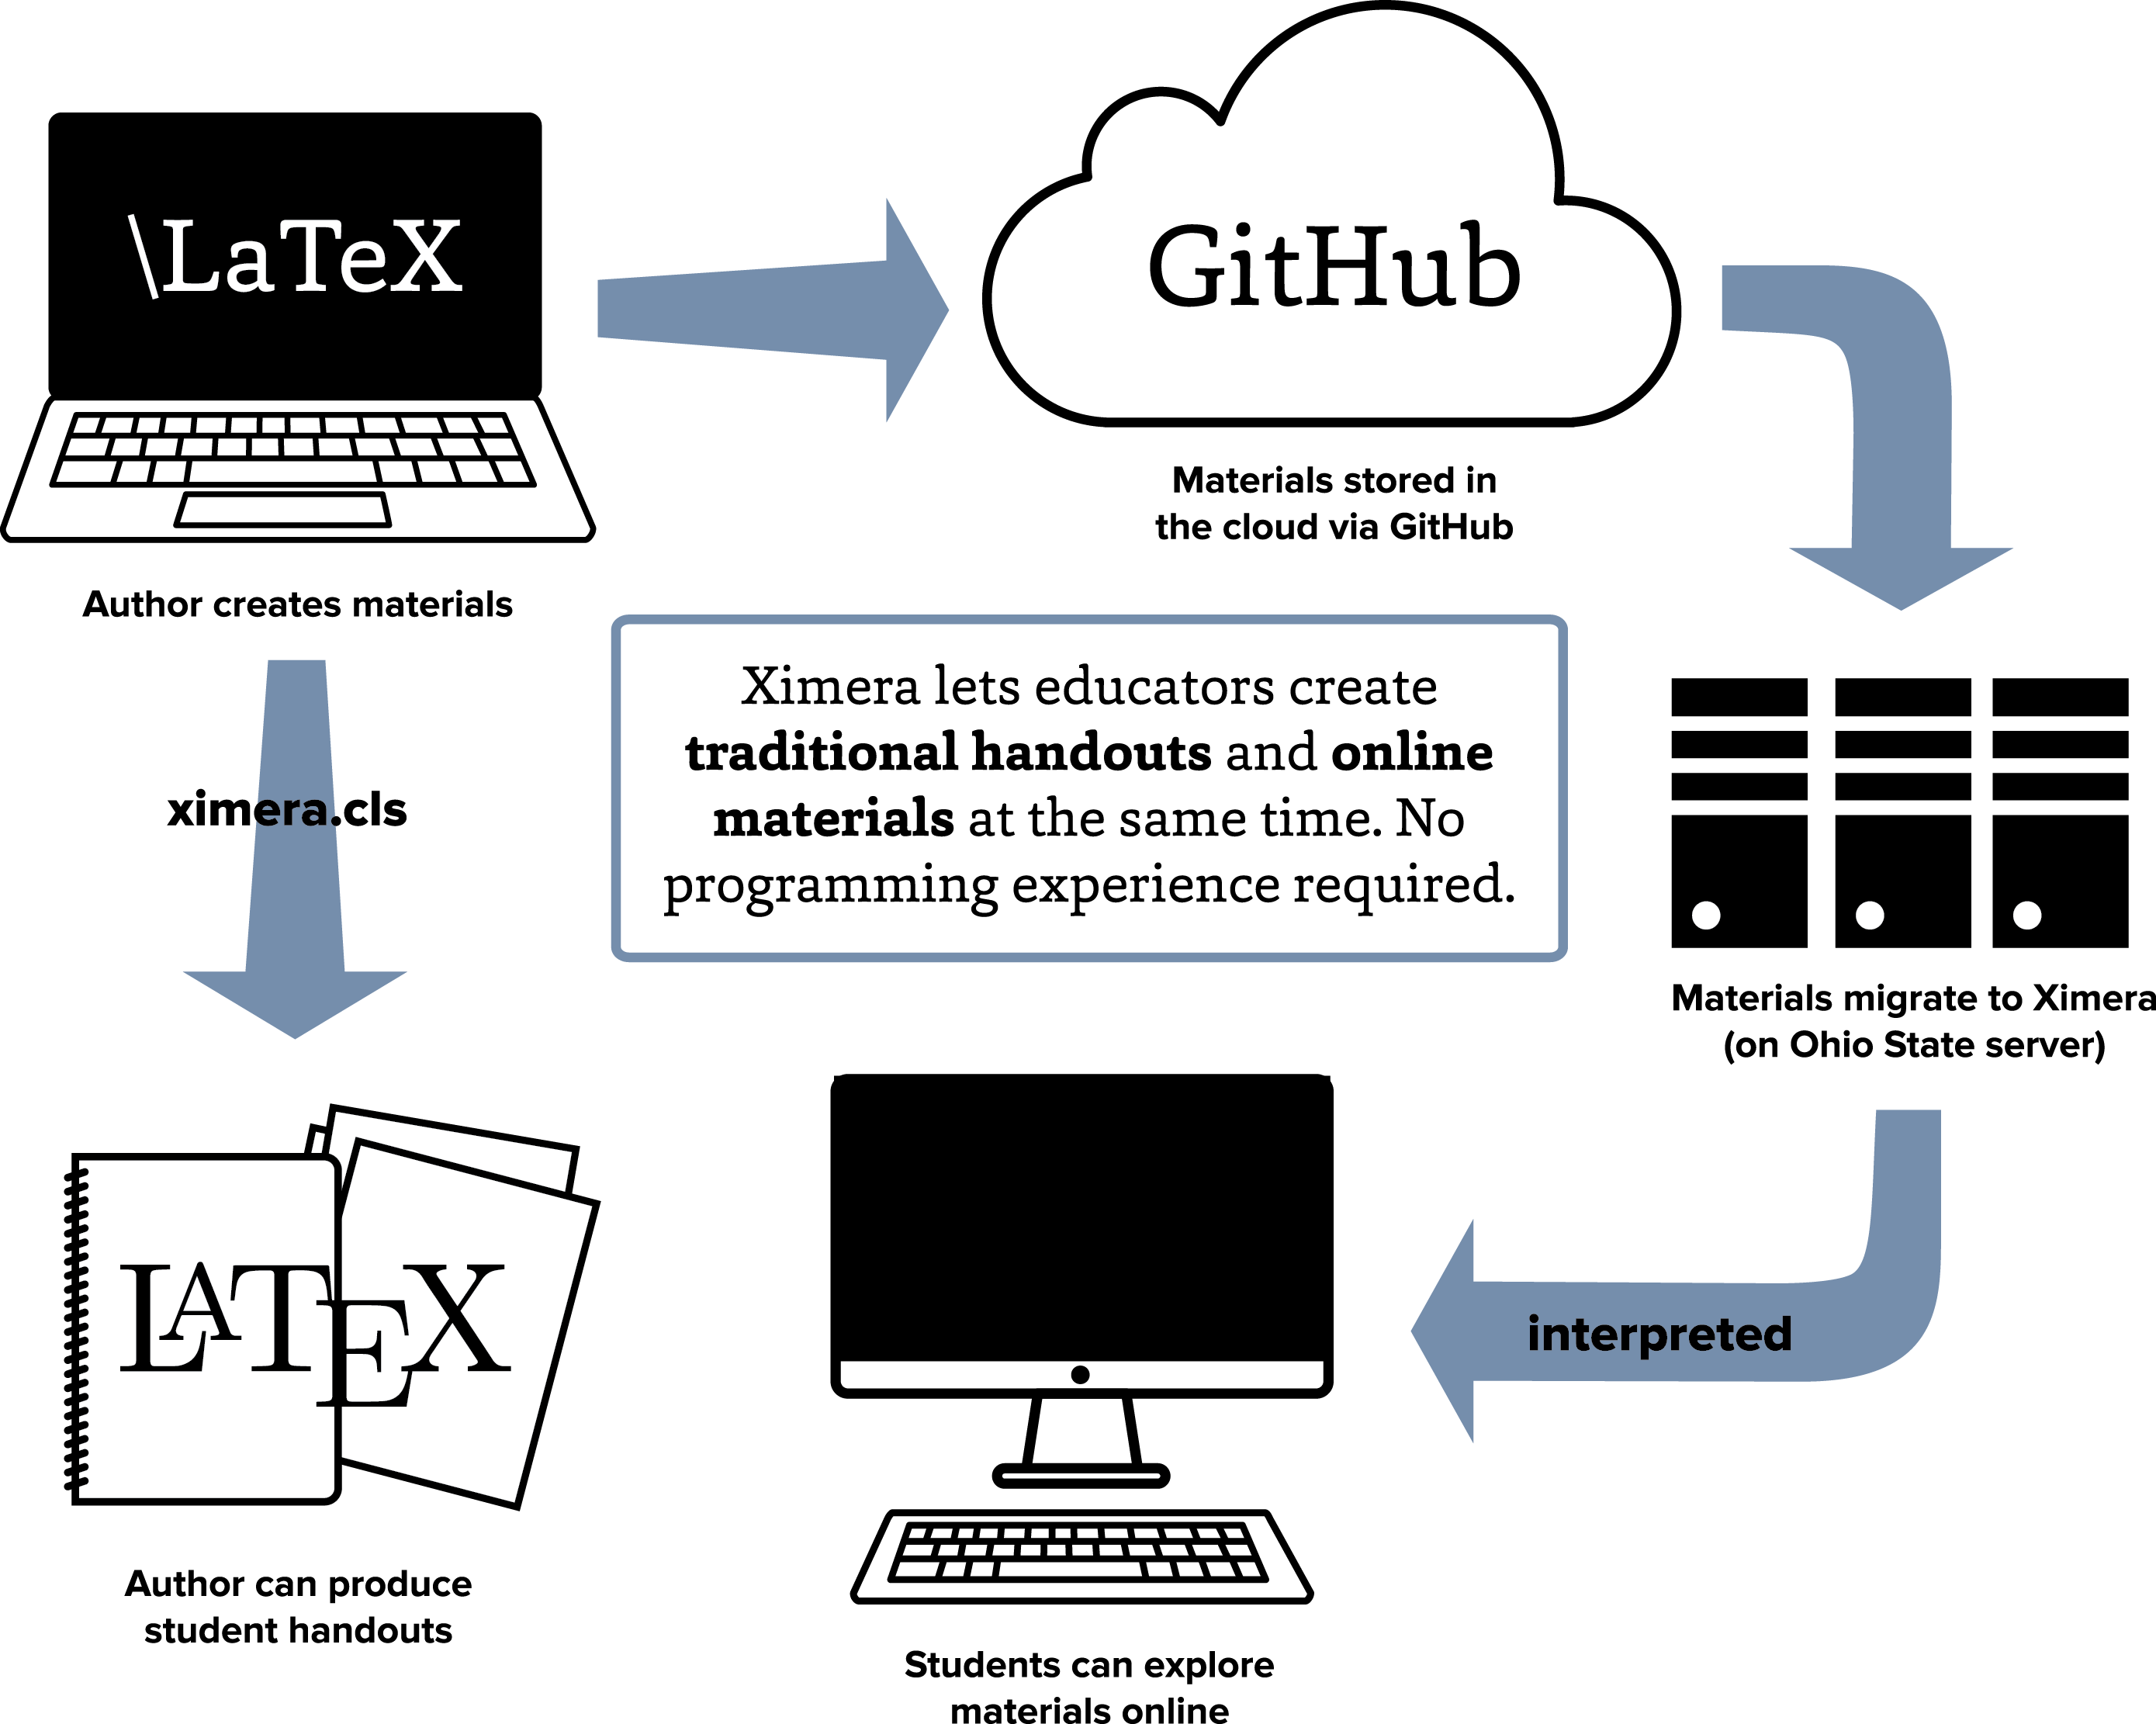
\includegraphics{XimeraGraphic.png}
\end{image}

\begin{enumerate}
\item Create a directory for your course files
and change to that directory.
In this example, we will create a directory called \verb!sampleCourse!.
Open a terminal session and issue the following commands:
\begin{center}
\begin{verbatim}
mkdir sampleCourse
cd sampleCourse 
\end{verbatim}
\end{center}
\item A Ximera course consists of a directory (which we created above)
containing a text file called \verb!course.xim!. 
We will create a course that has only one activity.
Using any text editor,
create a file named \verb!course.xim! containing the content below:

\begin{verbatim}
---
name: Getting Started with Ximera
description: This is a Ximera activity explaining how to get started
with Ximera for course instructors.
---

example/example
\end{verbatim}

\begin{remark}
This file contains information such as
the name of the course, a description of the course,
and the names of all the \LaTeX\ activity files 
comprising the course, in the order
that they should be presented to students.
The \verb!course.xim! file above specifies that 
there is one activity file 
and that it will be located in \verb!example.tex!
written without the extension \verb!.tex!. 
In general, the syntax is \verb!path/to/the/texfile!.
We will
create this file in the next step.


Generally courses should have more than one activity,
with each activity filename appearing in \verb!course.xim!
without the \verb!.tex! extension and
indented to reflect its position in the course hierarchy.
We recommend placing each
activity in its own directory, which should have the same name.
This facilitates
sharing activities between collaborators and makes reusing existing
activities easier.
%Later in this course, we will see examples of
%how to borrow existing activities from other courses
%rather than starting from scratch. 
\end{remark}

\begin{warning}
Note that the file name must be \verb!course.xim! and 
the three dashes encapsulating the name and description
are required, as is the blank line following the second set of dashes!
\end{warning}

\item Create a new directory
in the \verb!sampleCourse! directory
called \verb!example! and
containing a file called \verb!example.tex!. 
\begin{verbatim}
mkdir example
cd example
touch example.tex
\end{verbatim}

\item Using your text editor, open \verb!example.tex!
and add the following content.
\begin{verbatim}
\documentclass{ximera}
\title{The First Activity}
\begin{document}
\begin{abstract}
This activity deals with \verb!Ximera! activities
\end{abstract}
\maketitle
\end{document}
\end{verbatim}

\begin{remark}
An activity should be in the document class \verb!ximera!
and should contain the title of the activity
and an abstract.
The activity above has at this stage
a title and abstract, but is otherwise blank.
\end{remark}

\item Log into your \href{http://github.org}{\tt github.org}
account and
create a repository with the same name as your top directory
\verb!sampleCourse!
by clicking the \verb!+! by your account name, as shown
below.

\begin{image}
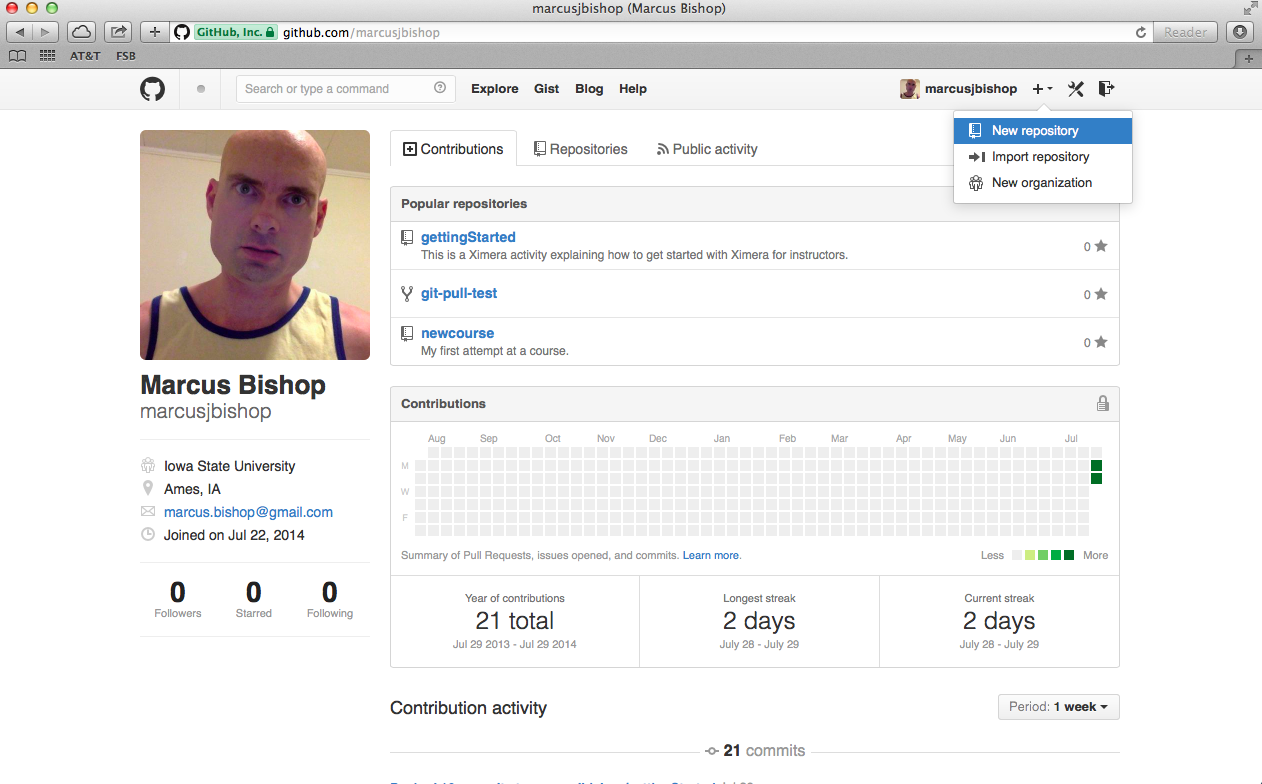
\includegraphics[scale=.3]{RepoInit.png}
\end{image}

Accept all default settings and press the
\verb!Create Repository! button
and \href{http://github.org}{\tt github.org}
will respond with additional directions shown below.
\begin{verbatim}
touch README.md
git init
git add README.md
git commit -m "first commit"
git remote add origin https://github.com/marcusjbishop/example.git
git push -u origin master
\end{verbatim}
Run the commands above.

\begin{remark}
These commands initiliaze the repository on \href{http://github.org}{\tt github.org}
and also create a file named \verb!README.md!.
\end{remark}

\item This step is optional. Edit the \verb!README.md! file
and write a description of the course. 

\begin{remark}
The contents of this file provides a description of the course that will appear
only on the \href{http://github.org}{\tt github.org} site for the repository.
\end{remark}

\item Click on the \verb!settings! button on the
\href{http://github.org}{\tt github.org} repository page
and then on \verb!Webhooks & Services!
\begin{center}
\begin{image}
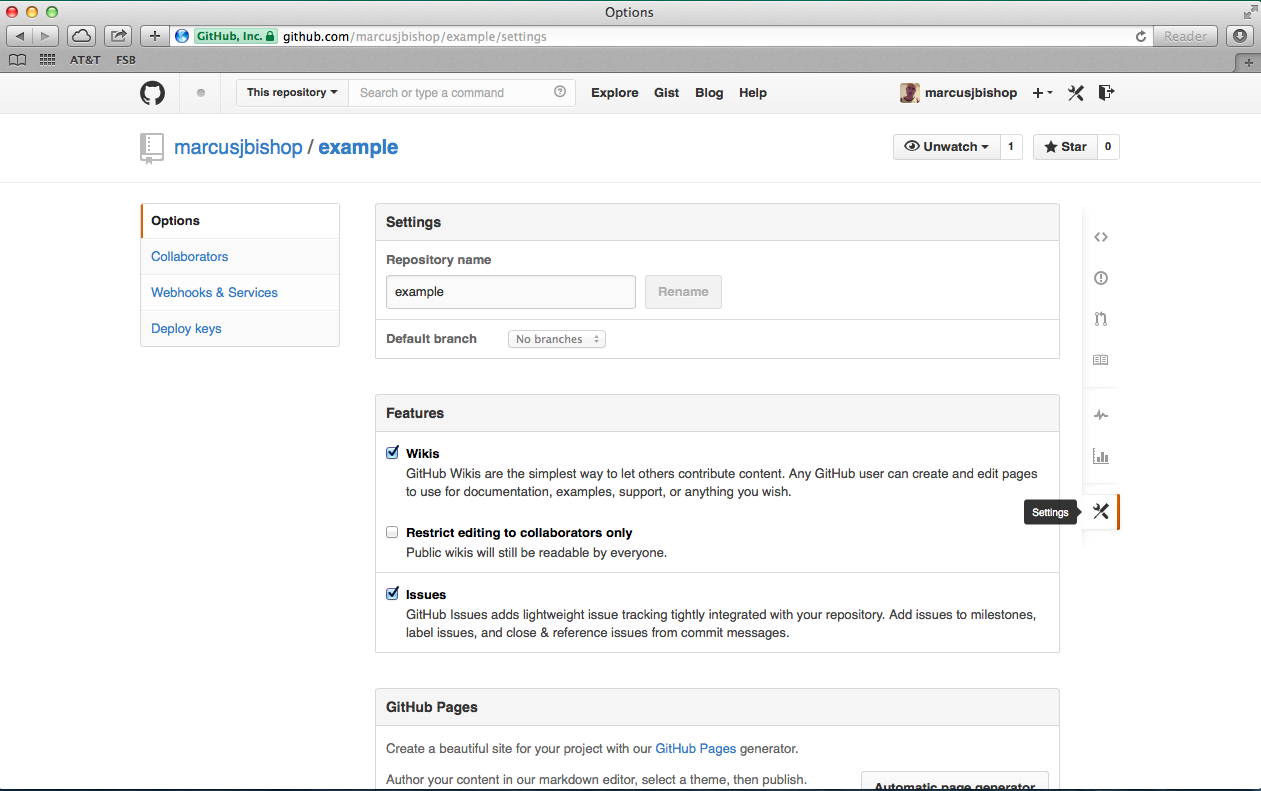
\includegraphics[scale=.3]{Webhook.png}
\end{image}
\end{center}
Now click the \verb!Add webhook! button.
Put \verb!http://ximera.osu.edu/github!
into the \verb!Payload URL! field and
\verb!8mi0tsrje9n3asPu86XC198G1XSdZj!
into the \verb!Secret! field.

\item In order to have your course listed on
\href{http://ximera.osu.edu/course}{\tt ximera.osu.edu/course}
you need to \verb!push! the repository.
However, since \verb!git! will not allow a \verb!push!
without any changes to the repository, this is a good point
to add content in the form of a simple exercise within the 
\verb!example.tex! file.
\begin{verbatim}
\documentclass{ximera}
\title{The First Activity}
\begin{document}
\begin{abstract}
This activity deals with \verb!Ximera! activities.
\end{abstract}
\maketitle
This activity is about creative work.
\begin{exercise}
  Choose the best place to work on mathematics.
  \begin{multiple-choice}
    \choice{At the library}
    \choice[correct]{At the caf\'e}
    \choice{In your office}
  \end{multiple-choice}
\end{exercise}
\end{document}
\end{verbatim}
See the following activity for more information on creating
exercises.

\item Change to the root directory of your repository
and execute the following commands.
\begin{verbatim}
git commit -am "Added an exercise"
git push
\end{verbatim}

\item If everything went well, you should find your course listed at 
\href{http://ximera.osu.edu/course}{\tt ximera.osu.edu/course}.
If not, see the troubleshooting activity
or send your questions to
\href{mailto:ximera@math.osu.edu}{\tt ximera@math.osu.edu}.
\end{enumerate}
\end{document}
